\section{Generazione degli eventi mockup con ChatGPT}
Per fornire una dimostrazione del sistema abbiamo caricato nel database una decina di escursioni di esempio.
La generazione di mockup di buona qualità generalmente richiede molto lavoro manuale affinché rispecchino la forma dei dati
che nel mondo reale verranno forniti alla piattaforma. Se si usano, per esempio, stringhe troppo corte o troppo lunghe si rischia di creare
un prodotto non adatto al mondo reale.
Nell'ultimo anno sono emersi numerosi Large Language Model (LLM) che si rivelano molto efficaci nella rielaborazione di testi, specialmente quando gli viene 
fornito un esempio su cui lavorare. Il nostro problema di generazione dei mockup è appunto un'istanza di questo problema che si presta molto bene ad essere
risolta dal un LLM\@.Abbiamo scelto di lavorare con ChatGPT essendo uno dei modelli più accessibili e prestanti al momento disponibili.\\ \\
Il primo passo è stato elaborare un prompt adeguato alla situazione che ``spiegasse alla macchina'' il problema che volecamo risolvesse e le fornisse un esempio
scritto da noi su cui lavorare (Figura~\ref*{fig:prompt1} e Figura~\ref*{fig:prompt2}).
\begin{figure}[ht]
  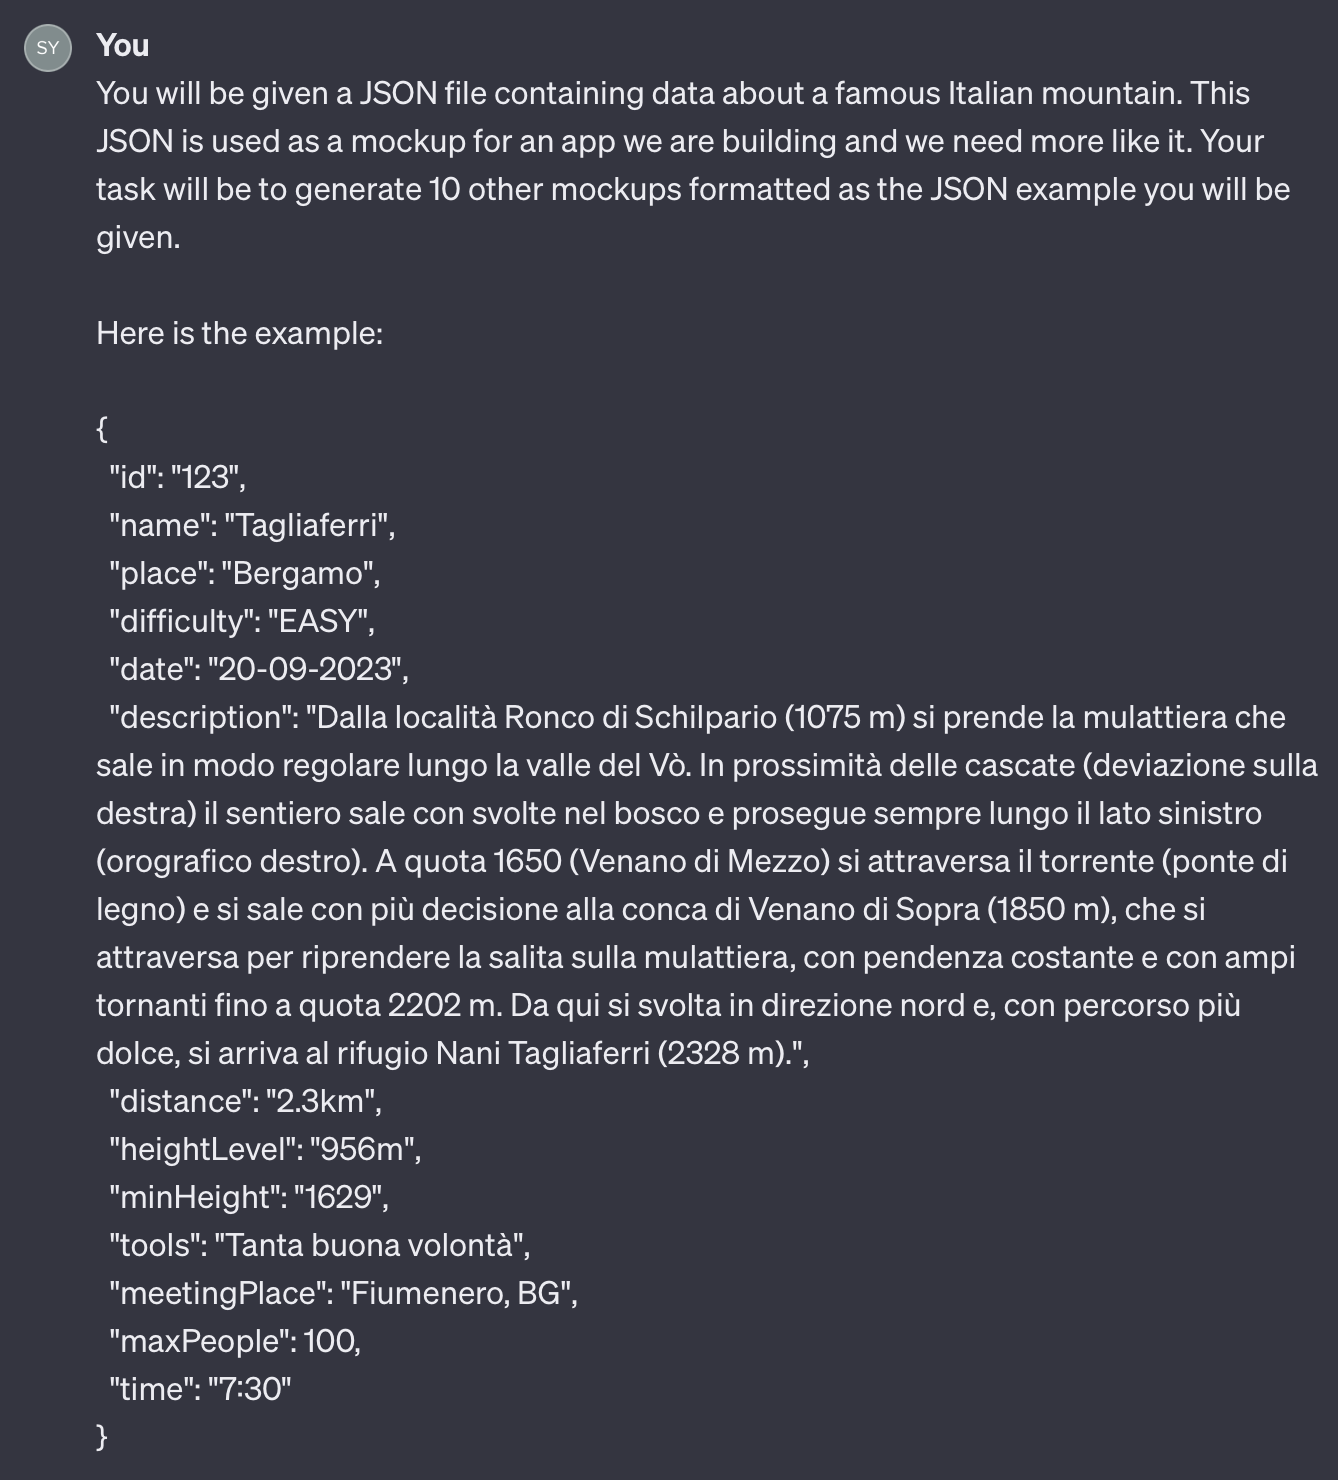
\includegraphics[width=\linewidth]{images/prompt1.png}
  \caption{Primo prompt}\label{fig:prompt1}
\end{figure}
\begin{figure}[ht]
  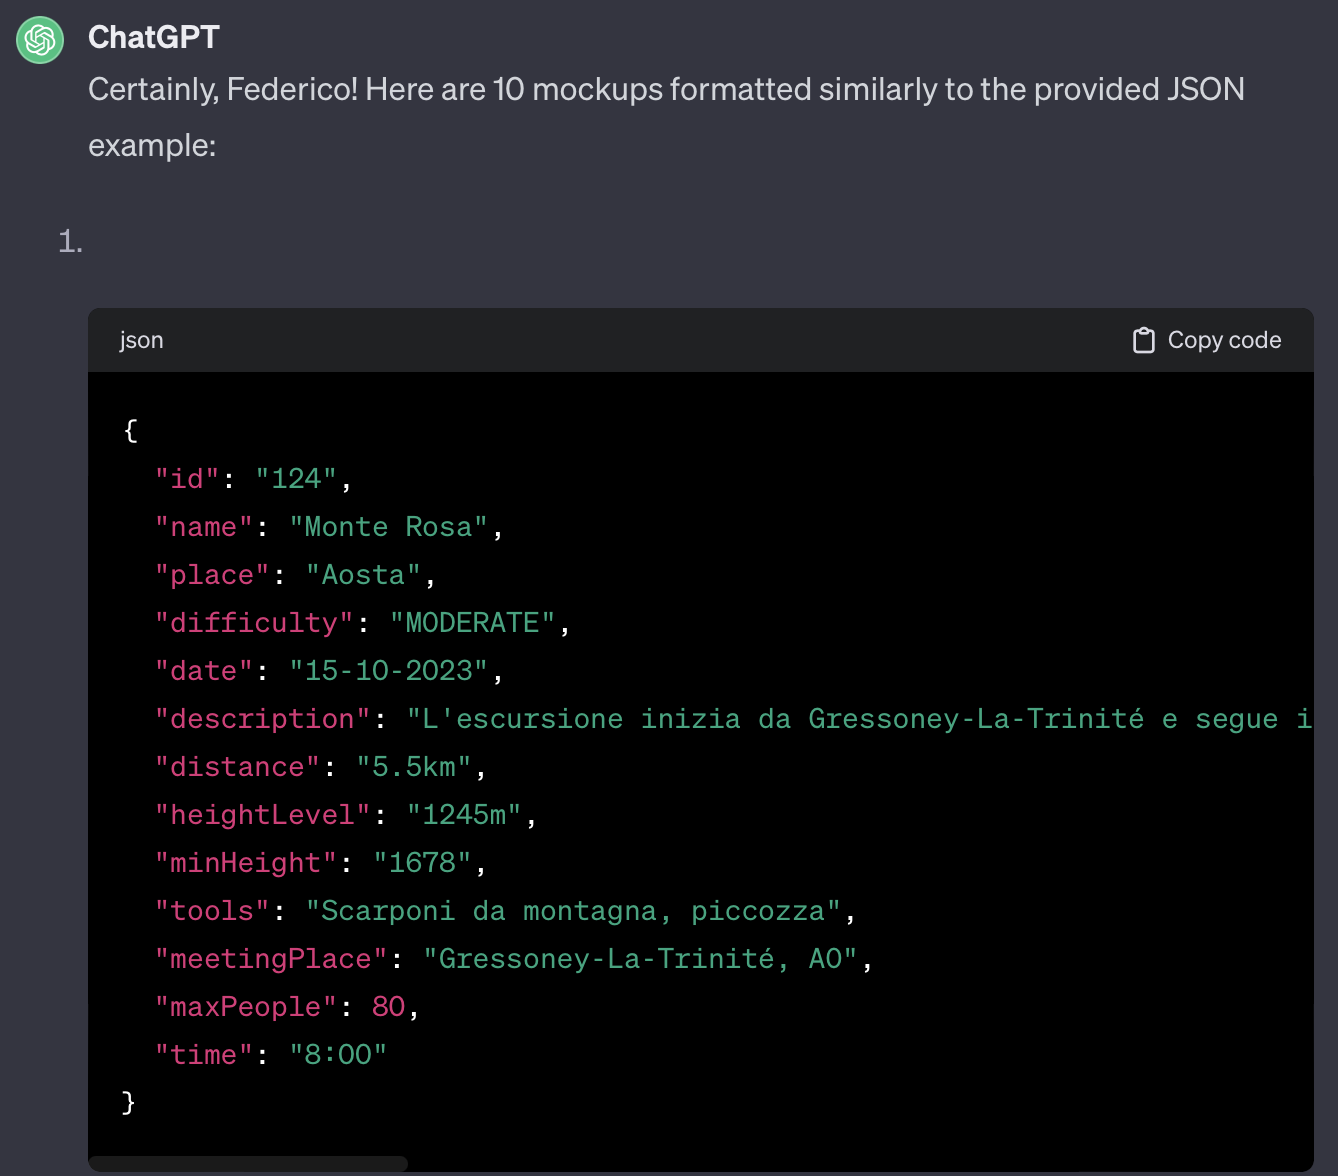
\includegraphics[width=\linewidth]{images/prompt2.png}
  \caption{Risposta parziale al primo prompt}\label{fig:prompt2}
\end{figure}
Successivamente abbiamo affinato il prompt fornendo dettagli più precisi sulla forma di ``difficulty'' (Figura~\ref*{fig:prompt3}).
\begin{figure}[ht]
  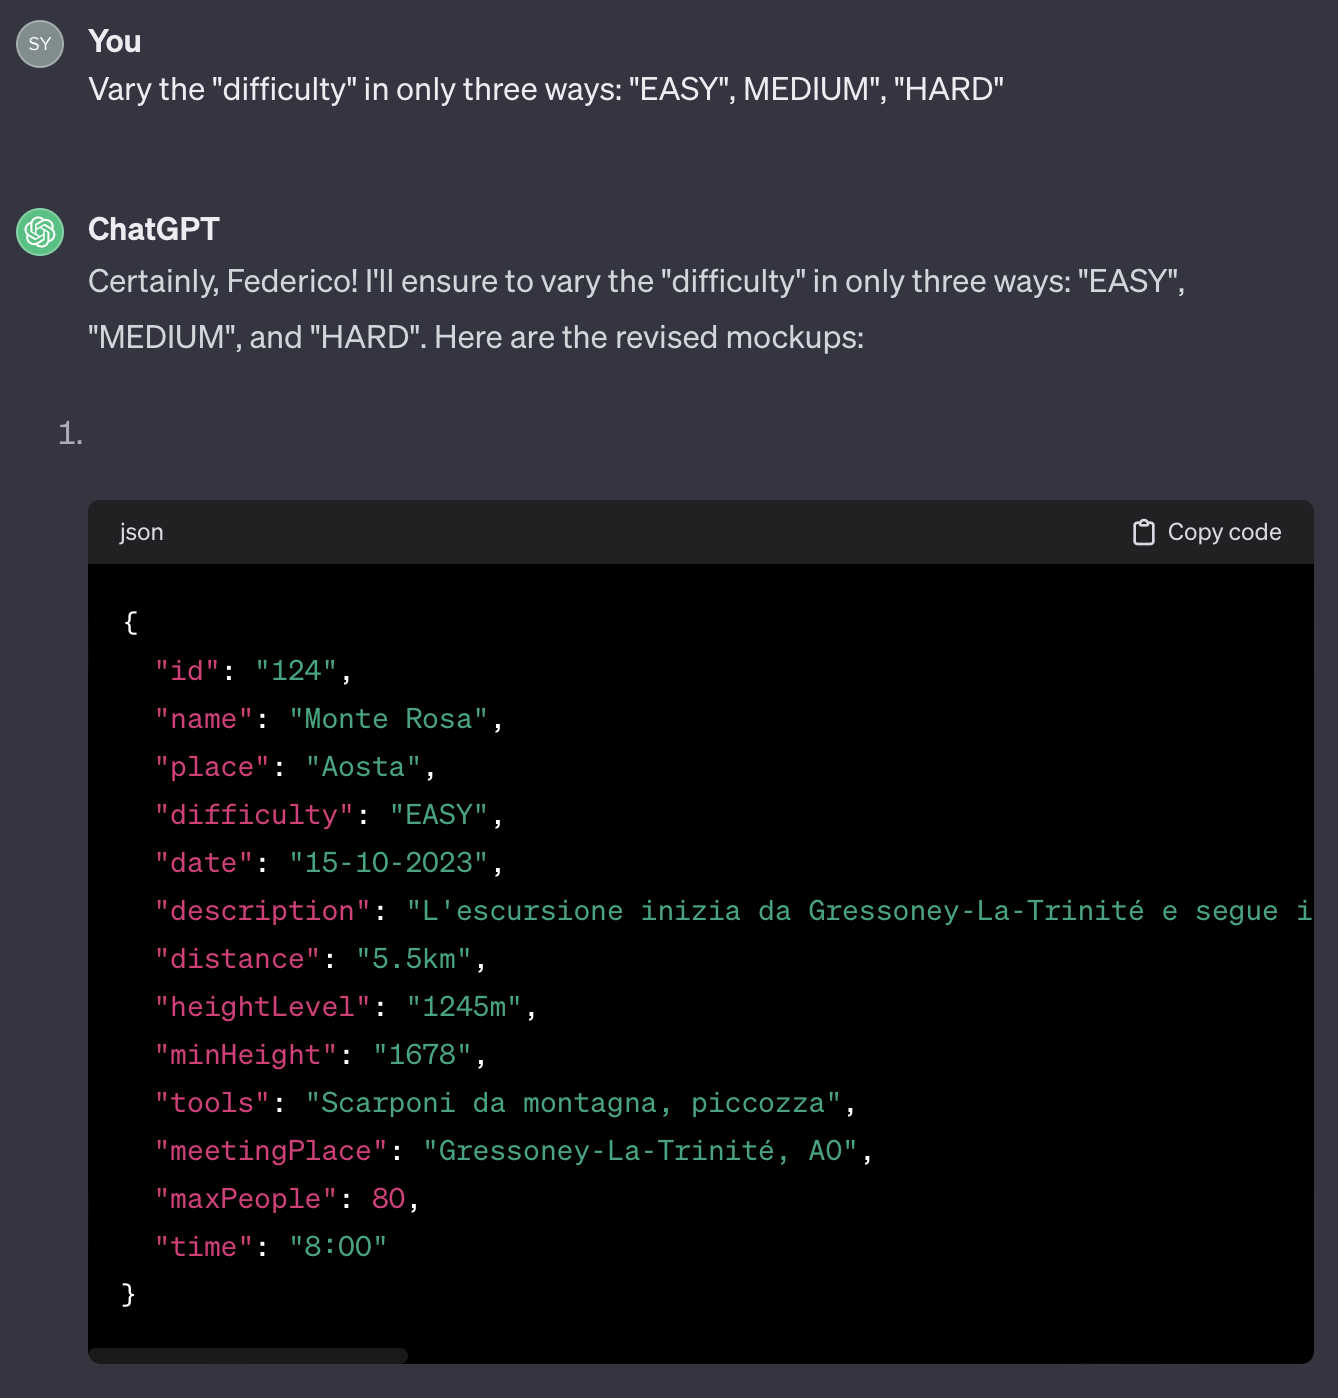
\includegraphics[width=\linewidth]{images/prompt3.png}
  \caption{Secondo prompt e risposta parziale}\label{fig:prompt3}
\end{figure}
Infine abbiamo chiesto che fossero generati i restanti mockup per arrivare a 10 (Figura~\ref*{fig:prompt4})
\begin{figure}[ht]
  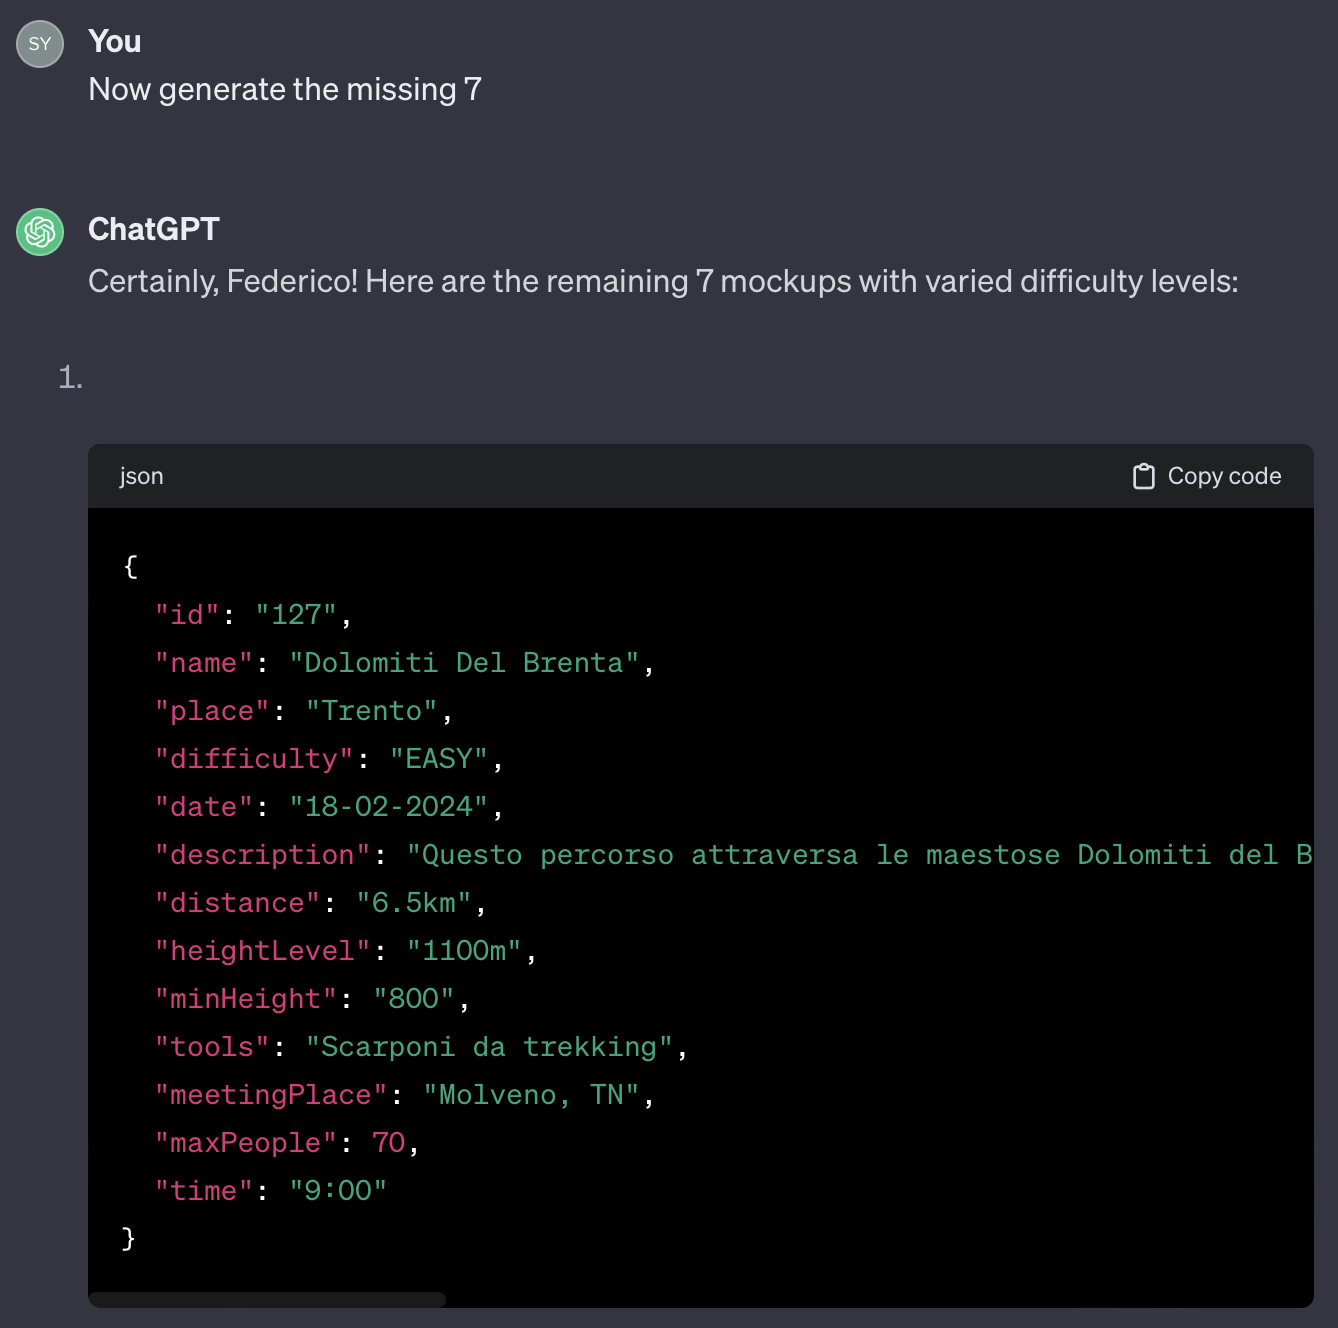
\includegraphics[width=\linewidth]{images/prompt4.png}
  \caption{Terzo prompt e riposta parziale}\label{fig:prompt4}
\end{figure}